\section{The Rubin Documentation Portal}
\label{sec:DocPortal}

The Documentation Working Group recommends the creation of a \emph{documentation portal} web application as a means of making documentation content discoverable and accessible to Rubin Observatory staff.
This documentation portal will provide interfaces for both searching (based on content and metadata) and browsing (based on hierarchical categorization) of documentation resources.
Documentation does not reside within the portal itself.
Rather, the portal's objective is to efficiently link the user to the document, where it is stored in any of the observatory's adopted storage platforms (Section~\ref{sec:primary-sources}).
The new Documentation Portal discussed herein is based upon the website \href{www.lsst.io} \citep{lsst.io-cite} which provides a search and browsing interface for the Rubin Observatory's public-facing technical documentation operated by the SQuaRE (Data Management) team.
(A detailed description of \href{www.lsst.io}, LSST the Docs (LTD) and applicable software is available in \citedsp{SITCOMTN-012}.)
The new portal will be accessible only those with Rubin Observatory staff credentials, and will be purpose-built for observatory and survey operations.
This section describes the design principles, technical architecture, security model, and cost estimate of the Rubin Observatory Documentation Portal.

\subsection{Design drivers}

The following are high-level design drivers for the future-state Rubin Documentation Portal. 
They reflect the recommendations made by the Documentation Working Group presented in this report.

\textbf{The role}  of the Documentation Portal is to link to documentation resources.
  The portal itself does not host the content itself, nor provide user interfaces for creating and maintaining new versions of documentation content.
  This requirement reflects the Documentation Working Group's recommendation that documentation content should be hosted on a select set of platforms that are idiomatic for the content and the teams that work with that content (Section \ref{sec:primary-sources}).

The Documentation Portal must provide equal support for content stored in any of the storage platforms (Section \ref{sec:storage-view}).

The Documentation Portal must be capable of supporting several hierarchical browsing schemes for accessing content based on different organizational views of the documentation (Section \ref{sec:views}).

The Documentation Portal should automatically update and sort documentation content, to the greatest extent possible.
  In other words, curators should only need to maintain documentation in the document's storage platform, without any administrative action through the Documentation Portal's user interface or infrastructure.
  A consequence of this requirement is that the Documentation Portal should not persist information about a document that is not available from the document's own storage platform.

The Documentation Portal should be secured so that it is only accessible to users with Rubin Observatory staff credentials.

The Documentation Portal should not maintain fine-grained access control for specific documents or categories of documents.
  For secured documents, the portal relies upon the security mechanisms of the document's own storage platform.
  The portal should also reduce its metadata storage of confidential documents to ensure that content cannot be inferred from a search, for example.


\subsection{Technical architecture}

The architecture described here is based upon that which is already put into production with the \href{www.lsst.io} portal for public-facing documentation.
Starting from this working archetype relieves a great deal of technical risk and development from the new portal's implementation.
Both portals share the use of Algolia \citep{Algolia-cite} as a search back-end and Ook \citep{ook-cite} as a content indexing service.
The Documentation Portal will have an independent front-end to support the specific Access Views recommended by the Documentation Working Group (Section \ref{sec:access-view}).
The Documentation Portal will also use a separate instance of the Algolia database to eliminate any risks associated with leaking internal documentation to the public-facing \href{www.lsst.io} portal.

Figure \ref{fig:portal-architecture} depicts the components of the Documentation Portal.

\begin{figure}[hp!]
\centering
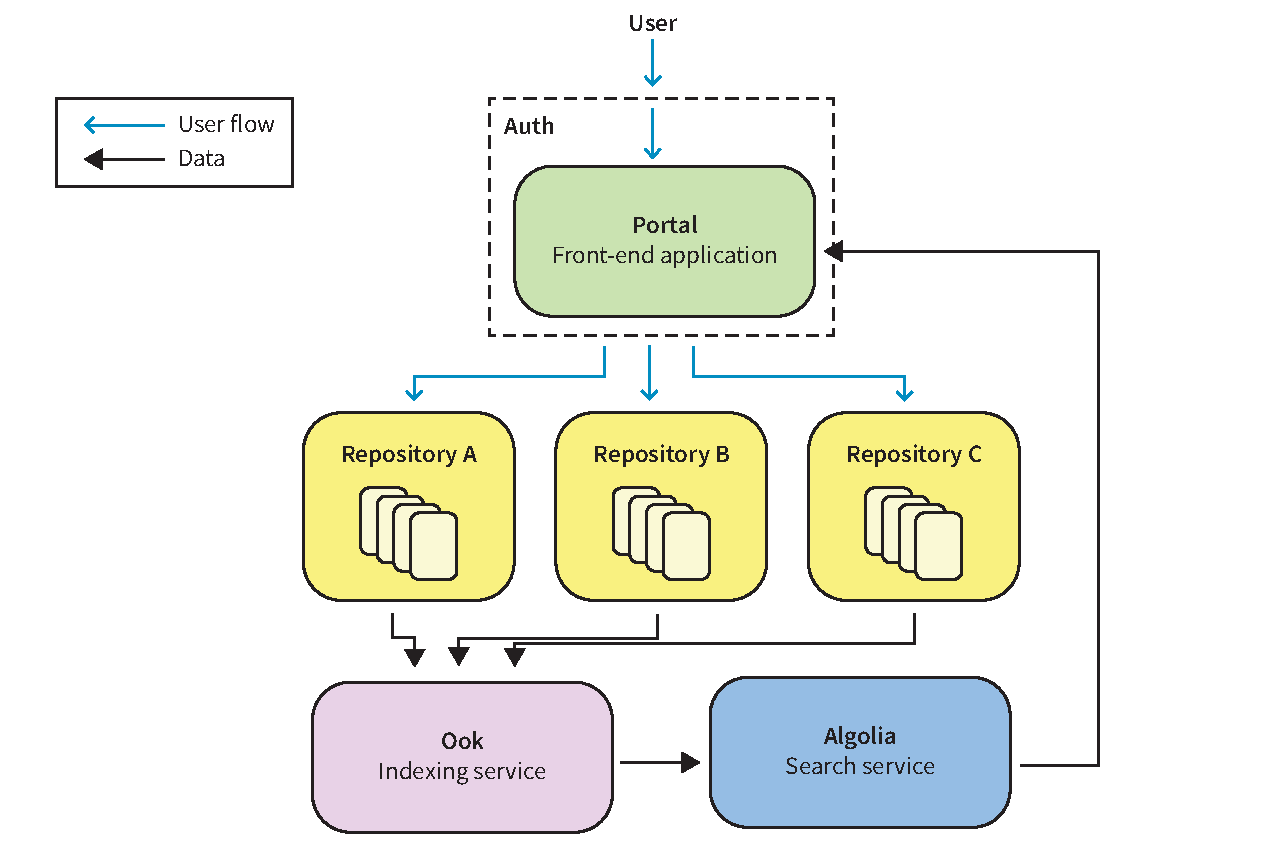
\includegraphics[width=0.95\textwidth]{portal-architecture}
\caption{Architecture of the Proposed Documentation Portal.
Users find documents on the web portal application, which in turn provides links into the original documentation repositories.
Data in the portal application is supplied by the Algolia search service \citep{Algolia-cite}, which in turn gets its metadata from the original documents in their repositories via the Ook indexing service \citep{ook-cite}.}
\label{fig:portal-architecture}
\end{figure}

\paragraph{Algolia}

The core function of the portal is to enable access to documentation through browsing and search.
To implement this, the portal needs a back-end service that contains metadata about Rubin Observatory's documentation holdings and provides interfaces to access and query that metadata from the front-end (i.e., the website).
This search database and interface could be made for "free" with entirely open-source components such as Elasticsearch \citep{elastic-cite} and in-house web service.
However, a search database and service are sufficiently generic that we cannot add value by making it in-house, and in fact developing, tuning, and operating this service, would costly in terms of labor.
For the \href{www.lsst.io} public documentation portal, we opted to use Algolia and recommend that we make the same choice for the new Documentation Portal.

Although \href{www.lsst.io} is currently operating on a free open-source license of Algolia, the new internal Documentation Portal would be an entirely paid license.
Algolia prices based on record counts and request rates.
In operating \href{www.lsst.io}, we found record count to be the limiting factor.
At the moment, $1,000$ records costs \$1 per month.
$1,000,000$ records would cost \$850 per month with volume discounts.
For reference, the \href{www.lsst.io} service currently uses $110,000$ records to host all technical notes and change-controlled documents with drafts hosted on LSST the Docs (LTD), also known as lsst.io.

Note that a single document is composed of potentially as many records in Algolia.
To optimize full-text search, we break a document into smaller records, generally across section boundaries.
Our current algorithms generally produce small record, so it is possible to reduce costs by tuning how we segment content into Algolia records.
Furthermore, each sorting option requires a separate pre-sort index.
Sorting documents by date, and document number, in addition to relevance, consumes three times as many records as only sorting by relevance.

\paragraph{Ook}

The Ook service is responsible for continuously indexing content into Algolia. \citep{ook-cite}
Whereas we chose Algolia to provide a turn-key search database service, for \href{www.lsst.io} we chose to build the indexing service in-house to have complete control over how documents are indexed, and what metadata is associated with each document.
For example, LaTeX-based documents are indexed based on metadata exported from the Lander PDF landing page generator (also developed in-house), which in turn parses LaTeX syntax in the document source to access metadata such as titles, authors, and so on.
The configurability of Ook is beneficial to indexing other types of highly specialized documentation.

The key design principle of Ook is that metadata is extracted from the document as it appears in its repository, rather than requiring direct human interaction with Ook or Algolia to curate the data.
This allows Ook to scale well across an organization as large and varied as Rubin because individual teams manage documents as they already do in the repositories they are already familiar with.

Ook is built such that new content types can be added by writing additional Python-based workflows for each content type.
Ook itself provides utilities for queuing ingests, converting content and formatting data for Algolia, and working with the Algolia service itself.

Ook indexing operations can be triggered several different ways.
For example, the lsst.io service publishes messages to a Kafka cluster whenever documentation is published on that platform; Ook subscribes to those messages and queues indexing workflows.
Ook indexing operations can also be scheduled through an HTTP API.
Generally, the goal is to trigger indexing operations automatically whenever the source material changes.

The existing Ook indexing workflows work by downloading content from websites and web services (HTTP APIs).
If content is not easily accessible, it would be possible to develop an alternative workflow, such as submitting copies of the document directly to Ook for indexing.
Some document repositories may offer online access but have hard-to-use APIs, DocuShare being a prime example.
These difficulties can be worked around, for example by emulating a web browser to download content and metadata, but at the cost of more fragile indexing workflows.

Ook is currently operated as a Kubernetes application in the Google Cloud.
This arrangement is ideal for minimizing operations cost, and providing convenient scaling.

\paragraph{Front-end application}

The front-end web application is how users (Rubin Observatory staff) find documentation.
The web application does not provide the document itself—instead, the web application provides a search result card that the user can click on to access the document in its original repository.
The Algolia services provides all browsing and search functionality; the front-end application provides the user interface over top of Algolia.

In addition to providing a link to the original document, the portal can also provide an immediate view of a document's metadata.
Although the front-end application can show a basic view of a document's metadata based on metadata common to all records, the website can be developed to show additional metadata for different types of documents.

For \href{www.lsst.io}, we built the site as a React JavaScript application.
This allowed us to use and customize the pre-made widgets provided by Algolia for building the user interface.

The front-end application will be accessible only to users who log in.
The simplest way to approach this is by putting the application behind a VPN so that the application is completely separate from security concerns.
Another approach would be to place the application behind an OAuth proxy to provide a slightly better user experience.

\subsection{Support for multiple views}

In Section \ref{sec:views}, the Documentation Working Group outlines several views for hierarchically arranging documents trees.
These views correspond to navigational structures in the front-end application.
Although the front-end application code is generally "aware" of the different trees, individual documents are placed in the tree on the basis of metadata in their Algolia records, so that the Algolia service can pre-sort and filter documents into the trees.
Since Ook supplies metadata to Algolia, and Ook in turn leverages metadata native to the document and the document's repository, the responsibility for curating documents into different views is the responsibility of individuals managing documents in each repository.

\subsection{Information security}

Documentation has multiple types of security concerns, such as control over who and how documents are updated, control over who can access documents, and ensuring the long term integrity and preservation of information.
Since the Documentation Portal is not the canonical repository for any documentation, the portal is not involved in controlling document updates and preservation.
The portal's key security concern is access control.

The portal is designed to only provide authentication-based access control.
Any Rubin Observatory staff member with credentials can access any metadata records contained within the Documentation Portal.
Once a user selects a document to view, they are forwarded to that documentation repository and must authenticate with that repository and be subject to its access control rules.

However, the metadata contained in the Documentation Portal can be potentially rich, even including the full-text content of a document to enable search functionality.
It is conceivable that some of this metadata may not be appropriate for observatory-wide access (such as information with export controls).
In these cases, the most realistic approach to preserving strict access controls in these situations is to limit what metadata is available.
In order of strictness, the following approaches can be used:

\begin{enumerate}
  \item Omit full-text content of a document from Algolia records.
  \item Limit or obfuscate other metadata (such as titles) in the Algolia records.
  \item Omit the individual documents altogether from Algolia and instead link to a documentation landing page hosted by the secure document repository itself.
\end{enumerate}

In all cases, controlling how documents are indexed is done by configuring the indexing service, Ook.
